\question[5]
Es sollen die starken Zusammenhangskomponenten des Graphen ermittelt werden.
Der im Unterricht vorgestellte Algorithmus ermittelt dazu eine
geeignete Reihenfolge, in der die Knoten des Graphen besucht werden. Die
jeweils erreichbaren Knoten bilden dann eine starke Zusammenhangskomponente.

a. Gib diese Reihenfolge der Knoten an
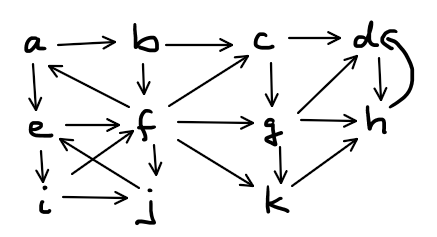
\includegraphics[height=5cm]{\pfad/Graphen/Aufgaben/scc_05/scc_05.png}
\begin{solutionbox}{2cm}
\begin{lstlisting}
d h k g c a f e j i b
\end{lstlisting}
\end{solutionbox}

b. Gib die Zusammenhangskomponenten in der Reihenfolge an, wie sie von
dem im Unterricht vorgestellten Algorithmus entdeckt werden.
Die Knotenreihenfolge innerhalb einer Komponente soll
alphabetisch geordnet sein.
\begin{solutionbox}{4cm}
\begin{lstlisting}
1 - d h
2 - k
3 - g
4 - c
5 - a b e f i j
\end{lstlisting}
\end{solutionbox}
